\section{Implementation specific for in-medium SRG}
\label{sec:ImplIMSRG}

Having explained the implementation for the free-space case, we will now proceed in a similar way for the in-medium implementation. This section will present all classes that are specific for the in-medium case, the algorithms we used and point out the steps we have taken to make the code as effective as possible, at the same time maintaining generalizability. 

\subsection{Classes for the in-medium case}

For consistency, we will present the relevant
classes  in a similar order as we did for the free-space case. First, we will present the two classes \textit{Hamiltonian} and \textit{Basis}, that are components of each \textit{System}. In particular, we will demonstrate how a smart arrangement of the basis can be used to store the matrix elements in a way that saves memory space of several orders of magnitude and at the same time 
leads to a considerable reduction of the problem's
dimension. Afterwards, we will turn to the implementation of the SRG method, performed by the class \textit{SRG}, and show how the structure of our basis also saves a great number of floating point operations when evaluating the flow equations.

\subsubsection{Class \textit{Basis}}

The purpose of the class \textit{Basis} is to create and administer a two-particle basis (tp-basis), meaning that one basis state is determined by two single-particle states (sp-states). For this idea, we have been inspired by \cite{Marte} and \cite{Christoffer}, since we made the observation that from a computational point of view, many routines of the SRG method resemble ones used in a Coupled Cluster implementation. Since M.H. J\o rgensen and C. Hirth demonstrated in their theses the enormous speed-up gained by such a  tp-basis, we decided to use a similar basis and storage system for the matrix elements, enabling us to make us of the obtained benefits.

Similar to the free-space case, one central data structure of the class \textit{Basis} is an array holding all sp-states for the number of considered shells $R$. As before, the items are of the type \textit{SPstate}, containing all quantum numbers, single-particle energy etc. At a later stage, we will demonstrate how this array is needed when setting up the tp-basis. \\
The core of the whole class \textit{Basis} are three arrays holding this basis. The idea is to have a mapping
\[
(M,M_s) \leftrightarrow \lambda,
\]
where $M = m_{(1)} + m_{(2)}$ and $M_s = m_{s(1)}+m_{s(2)}$ are the overall angular momentum and spin quantum number of the two particles, respectively. For each value of the so-called \textit{channel }$\lambda$, we tabulate those combinations of two sp-states that fulfil the requirements on $M$ and $M_s$. Hence, per two-particle state, we save the indices of two sp-states. Since needed later, we differentiate whether the indices lies above or below the Fermi level and therefore have three arrays: \textit{hhbasis} for both indices corresponding to holes lying below the Fermi level, \textit{ppbasis} for both indices corresponding to particles lying above the Fermi level and \textit{phbasis} if one of the indices lies above, the other one below the Fermi level. For efficiency reasons, i.e. to keep the basis as small as possible, we just store one of the possible combinations in the case that both indices refer to particles or holes.

\begin{lstlisting}[backgroundcolor=\color{lighter-gray},caption={\small Declaration of the three arrays saving the two-particle basis. Since we do not know the number of states in each channel in advance, we make use of the class \textit{vector} of the standard C++ library. The number of single-particle states, however, is always fixed to two, enabling us to use the type \textit{ivec2} of the Armadillo library.},numbers=none, label={lst:tp1}]
std::vector<arma::ivec2> *hhbasis, *ppbasis, *phbasis;
\end{lstlisting}

The algorithm for the mapping is based on the one by \cite{Marte} and demonstrated for the case of one particle and one hole in listing \ref{lst:tp2}. At an earlier stage of our program, the maximal M-value for two particles is computed as
\[
M_{max} = 2\cdot(R-1)
\]
and with
\begin{align*}
M &= 0,\pm 1, \pm 2,\dots,\pm M_{max} \\
M_s &= -1,0,+1
\end{align*}
the total number of channels $\lambda$ is
\[
lbd\_dim = 2\cdot M_{max}\cdot 3 + 3.
\]
In line 7 of listing \ref{lst:tp2}, we now allocate memory for storing the tp-basis for each possible channel $\lambda$. Then, we loop over all possible values for $M$ and $M_s$ to determine those two sp-states that fulfil the requirements for each channel. Since the demonstrated function creates the $ph$-basis, the first index $i$ must correspond to a particle, the second index $j$ to a hole. Using the quantum numbers stored in the array \textit{singPart}, containing all sp-states, we obtain $M$ and $M_s$ (see lines 19-20), and if they correspond to the ones of the current channel $\lambda$, we add the particle-hole combination to our basis (lines 24-25). For the $hh$- and $pp$-basis we proceed analogously.



\begin{lstlisting}[float, caption={Setting up the two-particle basis for the case of one particle and one hole. A detailed explanation can be found in the text.}, label={lst:tp2}]
void Basis::create_ph() { 
    ...
    int counter = 0;
    int lbd = 0;
    
    // Allocating space for each channel 
    ph_basis = new std::vector<arma::ivec2>[lbd_dim];
     
    // Loop over all possible values of M
    for (int l = -Mmax; l <= Mmax; l++) {
        channel(0) = l;
        
        // Loop over all possible values of M_s (since m_s is stored as integer, here -2,0,+2)
        for (channel(1) = -2; channel(1) <= 2; channel(1)+=2) {

            for (int i = hole_states; i < sp_states; i++)  // i = particle
                for (int j = 0; j < hole_states; j++) {  // j = hole

                    M = singPart[i].qnumbers[1] + singPart[j].qnumbers[1];
                    Ms = singPart[i].qnumbers[2] + singPart[j].qnumbers[2];

					// If channel is correct, add particle-hole combination
                    if (M == channel(0) && Ms == channel(1)) {
                        contr << i << j << endr; 
                        ph_basis[lbd].push_back(contr);
                    }
                }          
            lbd++;
        }
    }
}
\end{lstlisting}

Those three functions establishing the tp-basis constitute one group of functions in our class \textit{Basis}. Another group of functions is responsible to map between a certain particle and/or hole combination and the corresponding index in the two-particle basis. This will be needed later when we want to access a specific matrix element of the Hamiltonian.\\
All three functions are structured the way
\begin{align*}
\text{\textbf{Input: }}& \text{sp-index 1, sp-index 2, channel $\lambda$} \\
\text{\textbf{Output: }}& \text{index in tp-basis}.
\end{align*}
An example for the $ph$-basis is given in listing \ref{lst:tp3}. In functions of the class \textit{Hamiltonian}, using the tp-basis, we often have to loop over all basis states, which therefore should be as effective as possible. Studying Fig.\ref{fig:shellstructure}, it gets intuitively clear that just for the case of the $pp$-basis, all possible channels $\lambda$ are exploited. For the $ph$- and especially the $hh$-basis, a much smaller, central range is needed. To increase efficiency when looping over the states, we therefore save for each of the three bases the first and last occupied channel $\lambda$. An extract of the corresponding function, here for the $ph$-basis, is given in listing \ref{lst:tp4}.

\begin{lstlisting}[float, caption={Mapping between a pair of one particle and one hole and the corresponding index in the two-particle basis. For the case that the channel $\lambda$ is not known in advance, it can be obtained by the function \textit{get\_lbd}, which has to be provided with the quantum numbers $M$ and $M_s$ and returns the channel $\lambda$.}, label={lst:tp3}, numbers=none]
int Basis::map_ph(int p, int h, int lbd){ 
    
    for(int i = 0; i< ph_basis[lbd].size(); i++)
        if( (p == ph_basis[lbd][i](0)) && (h == ph_basis[lbd][i](1))){
            return i;
        }
    ...    
}

int Basis::get_lbd(int M, int Ms){ 
    return (M+Mmax)*3+(Ms/2)+1;  // Note: in our case Ms/2= {-1,0,1}   
}

\end{lstlisting}
 
\begin{lstlisting}[float, caption={Getting the first and last occupied channel $\lambda$, here an extract for the $ph$-basis. The boundaries are saved in an integer-matrix, which is returned by the function.}, label={lst:tp4}, numbers=none]
imat Basis::lbd_limits(){

    ...
    
    // Lower bound ph_basis
    lbd = 0;
    while(ph_basis[lbd].size() == 0)
        lbd++;   
    mat_ret(1,0) = lbd;
    
    // Upper bound ph_basis
    lbd = lbd_dim-1;
    while(ph_basis[lbd].size() == 0)
        lbd--; 
    mat_ret(1,1) = lbd;
    
    ...
}
\end{lstlisting}


\subsubsection{Class \textit{Hamiltonian}}

The task of the class \textit{Hamiltonian} is to set up the initial Hamiltonian matrix and administer the access to its elements.\\
The two central data structures are an object of type \textit{Basis}, by which the Hamiltonian communicates with the basis, as well as an array called \textit{mat\_elems}, which contains all the matrix elements.\\
Considering the computational parallels to Coupled Cluster calculations, we have, as mentioned before, been inspired by \cite{Marte,Christoffer} and save the elements in a special, effective way. 

First of all, we aim to make use of the symmetries of the Hamiltonian
\be
\langle p q || r s \rangle =  - \langle q p || r s \rangle = - \langle p q || s r \rangle = \langle q p || s r \rangle,
\label{eq:symmetry}
\ee
enabling us just to store one of four possibilities, which reduces the required memory space, and later also the number of flow equations, considerably. Second, we utilize that our two-body interaction is modelled by a Coulomb interaction, which is spherically symmetric and independent of spin. Therefore the angular momentum, as well as the spin, are conserved and we obtain an additional criterion for the two-particle elements $\langle p q || r s \rangle$:\\
Defining 
\begin{align*}
M &= m_{(p)} + m_{(q)}, \quad M' = m_{(r)} + m_{(s)}  \\
M_s &= m_{s(p)}+m_{s(q)}, \quad M_s' = m_{s(r)}+m_{s(s)},
\end{align*}
each two-particle state can be characterized by the two quantum numbers $M$ and $M_s$:
\[
| p q \rangle \leftrightarrow |M, M_s \rangle.
\]
Considering the conservation of quantum numbers, we then have
\[
\langle M,M_s | \hat{v}| M',M_s' \rangle = 0 \quad \text{if } M \neq M' \text{ or } M_s \neq M_s'.
\]
In other words, only transitions between two states of the same channel $\lambda$ yield a non-zero result, showing the purpose of our structure of the class \textit{Basis}. That way, we store the Hamiltonian in block-diagonal matrices, one block for each channel $\lambda$. To make us of the tp-basis and, furthermore, since the flow equations (\ref{eq:flow2order1})-(\ref{eq:flow2order}) depend on whether the indices correspond to particle or hole states, we differentiate between the following combinations
\begin{align}
v_{hhhh} &\corresp \langle i j |  | k l \rangle, \notag \\
v_{phhh} &\corresp \langle a j |  | k l \rangle, \notag \\
v_{pphh} &\corresp \langle a b |  | k l \rangle, \notag \\
v_{phph} &\corresp \langle a j |  | c l \rangle, \notag \\
v_{ppph} &\corresp \langle a b | | c l \rangle, \notag \\
v_{pppp} &\corresp \langle a b |  | c d \rangle,
\label{eq:vcombs}
\end{align}
where $p$ denotes particles above the Fermi level, $h$ holes below the Fermi level and, as before, indices $\lbrace a,b,c,d \rbrace$ and $\lbrace i,j,k,l\rbrace$ designate particle and hole states, respectively. These six combinations cover all basic possibilities for the interaction elements. For other ones, e.g. $v_{hphh}$, we exploit the symmetry relations (\ref{eq:symmetry}), obtaining
\begin{align}
v_{hhhh} &, \notag \\
v_{phhh} &= -v_{hphh} = -v_{hhhp} = v_{hhph}, \notag \\
v_{pphh} &= v_{hhpp}, \notag \\
v_{phph} &= -v_{hpph} = -v_{phhp} = v_{hphp}, \notag \\
v_{ppph} &= -v_{pphp} = -v_{hppp} = v_{phpp}, \notag \\
v_{pppp} &,
\label{eq:vsyms}
\end{align}
such that we have all $2^4=16$ possible combinations. Tabulating only the six matrices of Eq.~(\ref{eq:vcombs}), therefore provides all needed information.\\
The v-elements are stored in the tp-basis established in the class \textit{Basis}. As an example, take an element of the type $v_{phph} \corresp \langle a j |  | c l \rangle$. Since we store the Hamiltonian in block-form, the states $| a j\rangle$ and $|c l \rangle$ need to belong to the same channel $\lambda$. For each $\lambda$, the matrix $v_{phph}$ is of size $s_{ph(\lambda)}\times s_{ph(\lambda)}$, where $s_{ph(\lambda)}$ denotes the number of particle-hole combinations the $ph$-basis holds for this value of  $\lambda$. For a specific channel, the matrix element $v_{phph}(0,0)$ then contains the transition amplitude from the first to the first item in the corresponding $ph$-basis, the element $v_{phph}(0,1)$ the one from the first to the second, etc. 

For the f-elements of the Hamiltonian, see Eq.~(\ref{eq:felems}), we have the symmetry relation
\[
f_{pq} = f_{qp}.
\] 
To make use of this relation, we store the f-elements in three matrices:
\begin{align}
f_{hh} \corresp f_{ij}, \notag \\
f_{ph} \corresp f_{ai}, \notag \\
f_{pp} \corresp f_{ab},
\end{align}
with the same notation for the indices as before, and where $f_{hh}$ and $f_{pp}$ are symmetric such that only the upper triangular part has to be computed explicitly. Elements of the type $f_{hp}$ can be obtained via $f_{hp} = f_{ph}$.

In total, the complete Hamiltonian is stored in the array \textit{mat\_elems}, whose items are matrices, handled by the Armadillo library.
\begin{lstlisting}[backgroundcolor=\color{lighter-gray},numbers=none]
std::vector<arma::mat> mat_elems;
\end{lstlisting}
The first item of this array holds the ground state energy $E_0$, the three next ones the matrices $f_{hh}, f_{ph}$ and $f_{pp}$. The remaining items contain the v-elements. Starting with the lowest channel $\lambda$, we have for each channel the six matrices of Eq.~(\ref{eq:vcombs}).\\

To give an example of how this storage pattern reduces the required memory space by taking into account sparsity and symmetry relations, consider the case of $N=2$ particles and $R=15$ shells, corresponding to $110$ single-particle states. If stored in a straightforward way, with the \mbox{f-elements} in one two-dimensional and the v-elements in one four-dimensional matrix, one would need $110^4+110^2$ elements, corresponding to approximately $1.2$GB of memory. The required memory for our array, however, is only about $76$MB. The benefit is larger, the more shells $R$ the system includes. Apart from a  significant reduction of space in memory, the number of ODEs to be solved is thereby significantly reduced, too. 

To obtain access to a specific matrix element, the class \textit{Hamiltonian} provides appropriate functions, called \textit{get\_f\_elem} and \textit{get\_v\_elem}. Obtaining the f-element $f_{pq}$ is rather straightforward: Having determined whether the indices correspond to particle or holes states, the element can easily be extracted from one of the matrices $f_{hh},f_{ph}$ or $f_{pp}$, as shown in \mbox{listing \ref{lst:tp5}}.

\begin{lstlisting}[float, caption={Access to f-elements via the function \textit{get\_f\_elem}. The main idea is to determine which of the three possible matrices $f_{hh}$, $f_{ph}$ and $f_{pp}$ has to be used.}, label={lst:tp5}]
double Hamiltonian::get_f_elem(int p, int q, std::vector<arma::mat>& mat_elems) const {

    // f_hh
    if ((p < Bas->hole_states) && (q < Bas->hole_states))
        return mat_elems[1](p, q);

    // f_ph
    if ((p >= Bas->hole_states) && (q < Bas->hole_states))
        return mat_elems[2](p - Bas->hole_states, q);

    // f_hp
    if ((p < Bas->hole_states) && (q >= Bas->hole_states))
        return mat_elems[2](q - Bas->hole_states, p);

    // f_pp
    return mat_elems[3](p - Bas->hole_states, q - Bas->hole_states);

}
\end{lstlisting}

Accessing the v-elements is a bit more complicated since the elements are stored in the \mbox{two-particle} basis and according to channels $\lambda$. An excerpt of the function \textit{get\_v\_elem} can be found in listing \ref{lst:tp6}. 
To obtain a specific interaction element $v_{pqrs}$, the function
receives the four sp-state indices $p,q,r,s$. Inside the function, we first check whether the quantum numbers $M$ and $M_s$ are conserved, see lines 5-13. If not, the element has not been stored anyway, and we can return zero. Second (lines 15-23) we bring the indices into right order, since, as explained before, we only store one of the possible combinations for the $hh$- and $pp$-basis. If, for example, we have stored the combinations $|p_1 p_2\rangle$ and $| h_1 h_2 \rangle$ in our basis and are interested in the matrix element $v_{p_{2} p_1 h_1 h_2} = \langle p_2 p_1 | | h_1 h_2 \rangle$, we have to make use of the symmetry relations of Eq.~(\ref{eq:vsyms}) and ask for the element $v_{p_1 p_2 h_1 h_2}= - v_{p_2 p_1 h_1 h_2}$. \\
As a next step, we extract the right channel $\lambda$, see line 25. Knowing the channel and having the indices in the right order, we can access the matrix elements of our array \textit{mat\_elems}. However, the challenge is to extract which of the six combinations of Eq.~(\ref{eq:vcombs}) has to be used.  We therefore have to know explicitly, which of the indices correspond to hole and which ones to particle states. With this information, we can make use of the methods \textit{map\_hh}, \textit{map\_ph} and \textit{map\_pp} of the \textit{Basis}-class, yielding the index in the tp-basis and, finally, the element can be obtained. The many \textit{if-else} statements in listing \ref{lst:tp6} might look a bit clumsy, but enabled us to formulate the function in such a way, that we have as few checks concerning the correspondence to particle or hole states, as possible.\\
For our example $v_{p_2 p_1 h_1 h_2}$, we would now end up in the loop demonstrated in lines 49-53, where $p$ and $q$ are particles, and $r$ and $s$ are holes. There, the function \textit{map\_pp} gives the tp-basis index for $|p_1 p_2\rangle$, the function \textit{map\_hh} the one for $| h_1 h_2 \rangle$, and remembering the change of sign due to the ordering $|p_2 p_1\rangle \rightarrow |p_1 p_2\rangle$, the element can be accessed.

\begin{lstlisting}[float, basicstyle=\footnotesize, caption={Function for accessing the v-elements. See text for detailed explanation.},label={lst:tp6}]
double Hamiltonian::get_v_elem(int p, int q, int r, int s, std::vector<arma::mat>& mat_elems) const {
    ...   
    int sign = 1;

    int M1 = Bas->singPart[p].qnumbers[1] + Bas->singPart[q].qnumbers[1];
    int M2 = Bas->singPart[r].qnumbers[1] + Bas->singPart[s].qnumbers[1];

    if (M1 != M2) return 0; // Check conservation of momentum

    int Ms1 = Bas->singPart[p].qnumbers[2]+ Bas->singPart[q].qnumbers[2];
    int Ms2 = Bas->singPart[r].qnumbers[2]+ Bas->singPart[s].qnumbers[2];

    if (Ms1 != Ms2) return 0; // Check conservation of spin
 
    // Bring the indices into the right order
    if (p < q) {
        tmp = p;
        p = q;
        q = tmp;
        sign *= -1;
    }

    ... // The same for indices r and s
  
    int lbd = Bas->get_lbd(M1, Ms1); // Extract correct channel

    if (p < Bas->hole_states) {
        if (q < Bas->hole_states) {
            if (r < Bas->hole_states) {
                if (s < Bas->hole_states) {
                
                    // v_hhhh
                    comb1 = Bas->map_hh(p, q, lbd);
                    comb2 = Bas->map_hh(r, s, lbd);
                    if (comb1 < 0 || comb2 < 0) return 0; 
                    return sign * mat_elems[4 + 6 * lbd](comb1, comb2);
                } else {
                
                    // v_hhhp -> v_phhh
                    comb1 = Bas->map_ph(s, r, lbd);
                    comb2 = Bas->map_hh(p, q, lbd);
                    if (comb1 < 0 || comb2 < 0) return 0;
                    return -sign * mat_elems[5 + 6 * lbd](comb1, comb2);
                }
            } 
        } else { ...
            } else { ...
            ...
                    // v_pphh
                    comb1 = Bas->map_pp(p, q, lbd);
                    comb2 = Bas->map_hh(r, s, lbd);
                    if (comb1 < 0 || comb2 < 0) return 0;
                    return sign * mat_elems[6 + 6 * lbd](comb1, comb2);}
        }
    } 
}
\end{lstlisting}

Apart from storing the Hamiltonian matrix, the class \textit{Hamiltonian} is responsible for setting this matrix up. The v-elements can be stored the way they are, whereas the ground state energy $E_0$ and the f-elements have to be computed according to Eqs. (\ref{eq:gs2}) and (\ref{eq:felems}). 

\subsubsection{Class \textit{SRG}}
As explained for the free-space case, the class \textit{SRG} is the solver-class of our program.
 Given a \textit{System} with an initialized Hamiltonian, it solves the flow equations (\ref{eq:flow2order1})-(\ref{eq:flow2order}). Since the concrete terms for these flow equations depend on the generator $\hat{\eta}$, we designed the class \textit{SRG} as a virtual base class, similar to the class \textit{System}. It needs to be extended by subclasses for each used generator $\hat{\eta}$, containing the specific expressions for the flow equations, depending on $\hat{\eta}$. This procedure allows us to make use of the benefits that object-orientation in C{}\verb!++! offers: \\
 On the one hand, it gets uncomplicated to switch between different generators, on the other hand the program can easily be extended by further generators. In our case, we consider Wegner's and White's generator and have therefore implemented the corresponding subclasses \textit{Wegner} and \textit{White}.
  
\begin{figure}
\begin{center}
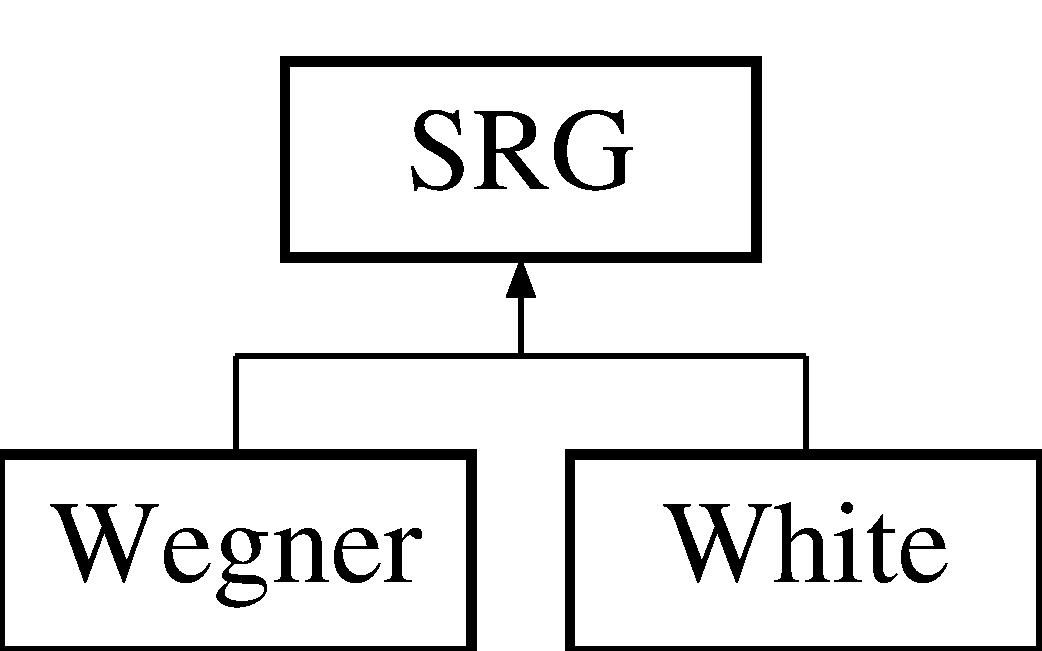
\includegraphics[scale=0.2]{../Plots/classSRG.pdf}
\caption{The class \textit{SRG} is a virtual  base class and needs to be extended by subclasses containing the specific expressions for the flow equations, depending on the generator $\hat{\eta}$.}
\label{fig:classSRG}
\end{center}
\end{figure}

The central data structures of the base class \textit{SRG} are an object of type \textit{System}, containing all system-specific information, as well as an array called \textit{eta}, where the values of the generator are stored during the integration. The size and structure of this array depend on the analytic expression of the generator and are specified in the subclasses.\\
The function \textit{run\_algo} performs the integration, using the ODE-solver of Shampine and Gordon. It is analogous to the free-space case, and concerning integration limits, step length etc., we therefore refer to subsection \ref{subsec:SRG}.

\subsubsection{Class \textit{Wegner}}

The class \textit{Wegner} is the subclass of \textit{SRG} which is designed for Wegner's canonical generator $\hat{\eta} = \left[ \Hd, \Ho \right]$. It extends \textit{SRG}, inheriting data structures and functions like the central function \textit{run\_algo}, and adds those parts that are generator-dependent. Dependency on the generator $\hat{\eta}$ occurs in two stages: First, for each integration step, the elements of $\hat{\eta}$ have to be updated and stored, then the derivatives (\ref{eq:flow2order1})-(\ref{eq:flow2order}) can be computed with these values. \\
In the following, we will explain those two stages in detail, including how elements are stored and accessed in our program. Afterwards we will demonstrate how we improved efficiency, both with respect to CPU time and memory.

\paragraph{Updating $\hat{\eta}$}
In principle, there exist two possibilities  to handle the generator $\hat{\eta}$ when computing the flow of the Hamiltonian: One possible way is to determine the elements under way, which means to start evaluating the flow equations (\ref{eq:flow2order1})-(\ref{eq:flow2order}) straightforwardly, and each time an element of $\hat{\eta}$ is needed, that one is computed according to Eqs. (\ref{eq:etaWegner1}) and (\ref{eq:etaWegner2}).
 The advantage would be not to use any memory for storing the $\hat{\eta}$-elements. 
 However, since the flow equations require many elements several times, lots of redundant calculations would be the consequence. 
 In fact, in one of our very first implementations to test the SRG method, we proceeded in such a way and realized that the redundant calculations made the program unacceptably slow. The second, now used approach for each integration step,  is to compute first all elements of $\hat{\eta}$, store them, and then continue with the derivatives using these elements. 

To store the $\hat{\eta}$-elements most efficiently, with an uncomplicated way of looping over and accessing them, we decided on the same structure as for the matrix elements of the Hamiltonian. The reasons are as follows:\\
First of all, the organization of the elements is similar, with the one- and two-body elements of $\hat{\eta}$ corresponding to the f- and v-elements of the Hamiltonian $\hat{H}$, respectively. Moreover, similar to the v-elements of $\hat{H}$, we aim to store the two-body elements $\eta_{pqrs}^{(2)}$ in our tp-basis. Since the generator, based on the Hamiltonian by $\hat{\eta} = \left[ \Hd, \Ho \right]$, conserves angular momentum and spin, too,  we intend to minimize memory for storage by saving $\hat{\eta}$ in the same block form. As a last motivation, required memory can further be reduced by making use of the relation $\hat{\eta}_s\da = -\hat{\eta}_s$, which apart from the sign is analogous to the symmetry of $\hat{H}$, giving the possibility to use the same storage system.\\
In analogy to the f-elements of $\hat{H}$, we save the one-body elements $\eta_{pq}^{(1)}$ in three matrices $\eta_{hh}^{(1)}, \eta_{ph}^{(1)}, \eta_{pp}^{(1)}$, depending on whether the indices correspond to particle or hole states. Elements of the form $\eta_{hp}^{(1)}$ can be obtained via $\eta_{hp}^{(1)} = -\eta_{ph}^{(1)}$. \\
For the two-body elements $\eta_{pqrs}^{(2)}$, we save analogous to Eq.~(\ref{eq:vcombs}) the six combinations
\begin{align}
\eta_{hhhh}^{(2)} &\corresp \langle i j | \hat{\eta} | k l \rangle, \notag \\
\eta_{phhh}^{(2)} &\corresp \langle a j | \hat{\eta} | k l \rangle, \notag \\
\eta_{pphh}^{(2)} &\corresp \langle a b | \hat{\eta} | k l \rangle, \notag \\
\eta_{phph}^{(2)} &\corresp \langle a j | \hat{\eta} | c l \rangle, \notag \\
\eta_{ppph}^{(2)} &\corresp \langle a b | \hat{\eta} | c l \rangle, \notag \\
\eta_{pppp}^{(2)} &\corresp \langle a b | \hat{\eta} | c d \rangle,
\label{eq:etacombs}
\end{align}
with the symmetry relations of Eq.~(\ref{eq:vsyms}) changed to
\begin{align}
\eta_{hhhh}^{(2)} &, \notag \\
\eta_{phhh}^{(2)} &= -\eta_{hphh}^{(2)} = \eta_{hhhp}^{(2)} = -\eta_{hhph}^{(2)}, \notag \\
\eta_{pphh}^{(2)} &= -\eta_{hhpp}^{(2)}, \notag \\
\eta_{phph}^{(2)} &= -\eta_{hpph}^{(2)} = -\eta_{phhp}^{(2)} = \eta_{hphp}^{(2)}, \notag \\
\eta_{ppph}^{(2)} &= -\eta_{pphp}^{(2)} = \eta_{hppp}^{(2)} = -\eta_{phpp}^{(2)}, \notag \\
\eta_{pppp}^{(2)} &.
\label{eq:etasyms}
\end{align}
The class \textit{Wegner} has two groups of functions concerning the generator $\hat{\eta}$: One group  is used to get access to the $\hat{\eta}$-elements, where the analogy to the matrix elements of $\hat{H}$ enabled us to use nearly the same functions, only modified by some signs. \\
The other important function is responsible for computing and storing the $\hat{\eta}$-elements in the corresponding array. The calculations are based on Eqs. (\ref{eq:etaWegner1}) and (\ref{eq:etaWegner2}), but for efficiency reasons split according to which indices correspond to hole and which to particle states. That way, we try to keep the number of floating point operations to a minimum and avoid computing
 contributions that are known to be zero in advance. As an example, the first term for the two-body elements $\eta_{pqrs}^{(2)}$, the term $f_{ps}v^d_{sqsq}\delta_{qr}$ of Eq.~(\ref{eq:etaWegner2}), can only give a contribution if $q$ and $r$ are both particles or holes. Therefore it needs not to be included for terms of the form $\eta_{pphh}^{(2)}$ and $\eta_{phph}^{(2)}$, and similar argumentations hold for the other terms of Eq.~(\ref{eq:etaWegner2}).


In order to test our implementation for $N=2$ particles against the exact result, and for easy extension from IM-SRG(2) to IM-SRG(3), we have opened up the possibility of including three-body terms of $\hat{\eta}$. The function
\begin{lstlisting}[backgroundcolor=\color{lighter-gray},numbers=none]
double SRG::get_eta3(int p, int q, int r, int s, int t, int u, std::vector<arma::mat>& mat_elems)
\end{lstlisting}
computes the elements $\eta_{pqrstu}^{(3)}$ following 
the commutation relations of Appendix \ref{App:AppendixB}:
\be
\eta_{pqrstu}^{(3)} = P(pq/r)P(s/tu)\sum_w \lb v^d_{pqsw} v_{wrtu} - v_{pqsw} v_{wrtu}^d \rb.
\label{eq:eta3order}
\ee
In order to avoid summing over terms that are known to be zero in advance, we have made 
use of the definitions of Eq.~(\ref{eq:diag}) and simplified the expression to
\begin{align}
\eta_{pqrstu}^{(3)} &= P(pq/r)P(s/tu)\lb v_{pqsq}v_{qrtu}\delta_{ps} + v_{pqsp}v_{prtu}\delta_{qs} \right. \notag\\
& - \left. v_{pqst}v_{trtu}\delta_{ru} - v_{pqsu}v_{urtu}\delta_{rt}\rb.
\label{eq:eta3orderSim}
\end{align}

\paragraph{Computing the derivatives}
The flow equations are in principle computed according to Eqs. (\ref{eq:flow2order1})-(\ref{eq:flow2order}), using the stored $\hat{\eta}$-elements in order to avoid redundant computations.  To keep the number of floating point operations to a minimum, we proceed similar to \mbox{updating  $\hat{\eta}$} and try to circumvent evaluating those terms that are known to be zero in advance. As we will demonstrate, this involves several adaptations of our code, making it sometimes a bit harder to read, but increases effectiveness enormously, which is crucial for the code's overall performance. 


\begin{lstlisting}[float, caption={Excerpt of the function \textit{E0\_deriv:}, which evaluates Eq.~(\ref{eq:flow2order1}). Here the second term of Eq.~(\ref{eq:flow2order1}) is demonstrated. For detailed explanation, see text.},label={lst:wegner1}]
for (int lbd = lbd_limits(0, 0); lbd <= lbd_limits(0, 1); lbd++)
      for (int ij = 0; ij < Sys->H->Bas->hh_basis[lbd].size(); ij++)
          for (int ab = 0; ab < Sys->H->Bas->pp_basis[lbd].size(); ab++)
                contr += -eta[6 + 6 * lbd](ab, ij) * mat_elems[6 + 6 * lbd](ab, ij);

    d_ret += 2 * contr;
\end{lstlisting}

To illustrate how we use our matrix elements with a tp-basis and how our classes work together, listing \ref{lst:wegner1} shows how the second term of Eq.~(\ref{eq:flow2order1}),
\be
\frac{1}{2}\sum_{ijab}\eta_{ijab}^{(2)}v_{abij},
\label{eq:E0term}
\ee
is evaluated in our program. In principle, the term loops over four indices: hole states $ \lbrace i,j \rbrace$ and particle states $\lbrace a,b \rbrace$. The tp-basis enables us to reduce the four loops to two loops, which for $N$ particles reduces the number of floating point operations from order $\mathcal{O}(N^4)$ to $\mathcal{O}(N^2)$: \\
Instead of summing over the two hole indices $\lbrace i,j \rbrace$, we loop over our \textit{hh\_basis}, as demonstrated in line 2 of listing \ref{lst:wegner1}. Furthermore, instead of summing over particle states $\lbrace a,b\rbrace $, we simply take all elements of our \textit{pp\_basis} (see line 3). Since term (\ref{eq:E0term}) sums over all indices $\lbrace i,j,a,b\rbrace$, we need to consider all channels $\lambda$ of the tp-basis, resulting in the additional loop of line 1. Since we loop over the $pp\_basis$ inside the loop of the $hh\_basis$, we can hold the number of considered channels $\lambda$ to a minimum by only taking into account the smaller range of the $hh\_basis$. \\
The contributions from the $eta$- and v-elements are added as shown in line 4, where we have to select the right two-body elements of Eqs. (\ref{eq:vcombs}) and (\ref{eq:etacombs}). In the case of term (\ref{eq:E0term}), this means to pick elements $\eta_{pphh}^{(2)}$ and $v_{pphh}$. For the first channel $\lambda$, these elements have been stored at the sixth position of the arrays \textit{eta} and \textit{mat\_elems}, respectively, afterwards the elements occupy every sixth position, due to six possible two-body elements. Hence, as listing \ref{lst:wegner1} shows, the indices of the required elements are accessed using the index $6+6*lbd$. 

The considerations about which of the possible elements in (\ref{eq:vcombs}) and (\ref{eq:etacombs}) have to be accessed, have not only to be made for term (\ref{eq:E0term}), but for each single term in the flow equations (\ref{eq:flow2order1})-(\ref{eq:flow2order}). This results often in splitting sums up to distinguish between particle and hole states and makes the code much more complex. However, as stated before, each loop over the tp-basis, instead of over two indices, reduces the number of floating point operations from $\mathcal{O}(N^2)$ to $\mathcal{O}(N)$, which is worth all extra work on the code.

Another advantage of our tp-basis is that for each of the two possible two-particle states $|pq\rangle$ and $|qp\rangle$, we only store one of the configurations. As can be seen in listing \ref{lst:wegner1}, we nevertheless sum only once over all elements in the tp-basis. The reason is that, due to symmetry relations (\ref{eq:vsyms}) and (\ref{eq:etasyms}), only  half of the indices has to be summed over, given that the final result is multiplied by two. Hence the tp-basis naturally halves the number of terms.

\paragraph*{Loop terms for IM-SRG(2/3)}
As explained for the implementation of the generator $\hat{\eta}$, our code has the possibility of including the loop terms of three-body interactions. With those loop terms we mean effective two-body terms of the form
\[
\langle p q || r s \rangle = \sum_i \langle p q i | v^{(3)} | r s i \rangle,
\]
and effective one-body terms of the form
\[
f_{pq} = \frac{1}{2}\sum_{ij} \langle p i j | v^{(3)} | q i j \rangle, 
\] 
where $i$ and $j$ sum over all hole states. To optionally include those terms, our implementation of the flow equations includes segments like listing \ref{lst:wegner2}, which gives the example for the derivative of the ground state energy $E_0$. The optional portions of the code are surrounded by a \textit{\#if} directive, determining during compile-time whether those lines of code are included or not.\\
Since our model of the Hamiltonian does not include three-body terms $W_{pqrstu}$ itself and we do not consider induced three-body interactions in IM-SRG(2/3), either, the rather complex Eq.~(\ref{eq:flow3}) reduces to the simple contribution
\be
\frac{d}{ds}v_{pqrstu}^{(3)} = \sum_v P(pq/r)P(s/tu) \lb \eta_{pqsv}^{(2)} v_{vrtu} - v_{pqsv} \eta_{vrtu}^{(2)}\rb
\label{eq:loopterms}
\ee
To stress the difference between IM-SRG(2/3) and IM-SRG(3) once more, we remind that \mbox{IM-SRG(3)} would require to store and consider all induced three-body interactions, involving the complete Eqs. (\ref{eq:flow0})-(\ref{eq:flow3}), whereas IM-SRG(2/3) simply extends the second order flow equations (\ref{eq:flow2order1})-(\ref{eq:flow2order}) by adding the loop terms to the f- and v-elements.

\begin{lstlisting}[float, caption={Optional inclusion of loop terms corresponding to three-body interactions, here the contribution to $dE_0/ds$.},label={lst:wegner2}]
#if SRG23
    for (int lbd = lbd_limits(0, 0); lbd <= lbd_limits(0, 1); lbd++)
        for (int ij = 0; ij < Sys->H->Bas->hh_basis[lbd].size(); ij++) {
            i = Sys->H->Bas->hh_basis[lbd][ij](0);
            j = Sys->H->Bas->hh_basis[lbd][ij](1);
            for (int k = 0; k < hole_states; k++)
                contr += get_dv3(i, j, k, i, j, k, mat_elems);
        }
    d_ret += (1.0 / 3.0) * contr;
#endif
\end{lstlisting}


\paragraph{Improving efficiency}
Compared to one of the first versions of our code, where we implemented the flow equations absolutely straightforwardly, we have obtained a speed-up of three orders of magnitude with our final code. This stresses how important optimization is to make the SRG method computationally affordable. Some of the means to improve efficiency have already been demonstrated, e.g. the use of the tp-basis, other ones concerning the class \textit{Wegner} will be shown in the following.

One especially useful tool is to express as many terms of the flow equations (\ref{eq:flow2order1})-(\ref{eq:flow2order})  as possible in terms of matrix-matrix multiplication. This often effectively reduces the number of indices to be summed over and enables us to profit from the highly optimized matrix tools of LAPACK and BLAS, which we access via the Armadillo library. \\
As an example, consider the term
\be
\sum_r \lb \eta_{pr}^{(1)} f_{rq} + \eta_{qr}^{(1)}f_{rp}\rb
\label{eq:fphterm}
\ee
of Eq.~(\ref{eq:flow2order2}) for the matrix of form $f_ {ph}$. In a first, straightforward approach, we expressed the term as shown in listing \ref{lst:wegner30}. The code segment is closely related to the mathematical equation and easy to read, but computationally ineffective since the elements are not accessed directly, but through getter-functions.

\begin{lstlisting}[float,caption={Term (\ref{eq:fphterm}) implemented straightforwardly, i.e. close to mathematical notation, and therefore easy to read.},label={lst:wegner30}]
for(int p_ind = 0; p_ind< part_states ; p_ind++){
       p = p_ind +hole_states;
        
       for(int q = 0; q < hole_states; q++){           
           for(int r = 0; r < all_states; r++)           
              dv[2](p_ind,q) += get_eta1(p,r)*H->get_f_elem(r,q,mat_elems) + get_eta1(q,r)*H->get_f_elem(r,p,mat_elems);
        ...
        }
}
\end{lstlisting}

A first step of optimization was therefore to reduce the number of calls to getter functions to a minimum and access elements, as often as possible, directly. We took this step of course not only in Eq.~(\ref{eq:flow2order2}), but in all functions dealing with arrays. To know exactly how to access the arrays, this involved making out for every single index whether this one corresponds to a particle or a hole state. Often this required sums to be split up, as demonstrated for our example (\ref{eq:fphterm}) in listing \ref{lst:wegner31}.\\ Apart from taking the right particle or hole indices, another demand is to pick the correct stored matrix by considering symmetry relations. For example, in the case that $r$ corresponds to a particle in term (\ref{eq:fphterm}), the element $\eta_{qr}^{(1)}$ needs to be transformed from the form $\eta_{hp}^{(1)}$ to $\eta_{hp}^{(1)} = -\eta_{ph}^{(1)}$. This use is demonstrated in line 15 of listing \ref{lst:wegner31}, where also the sign has been changed correspondingly.\\
As mentioned before, some expressions, like our example term (\ref{eq:fphterm}), even admit to be optimized further by using matrix-matrix multiplications. Considering basic matrix properties for the elements of $f_{ph}$, the contribution of term (\ref{eq:fphterm}) can be rewritten as
\begin{align*}
\sum_r \lb \eta_{pr}^{(1)} f_{rq} + \eta_{qr}^{(1)}f_{rp}\rb &\corresp \eta_{ph}^{(1)}\cdot f_{hh} + \lb \eta_{hh}^{(1)} \cdot f_{ph} \rb^T  \quad \text{(for hole states } r) \\
&+ \eta_{pp}^{(1)}\cdot f_{ph} - \lb \eta_{ph}^T \cdot f_{pp}, \rb^T \quad \text{(for particle states } r) 
\label{eq:fphmatrix}
\end{align*}
where '$\cdot$' denotes matrix-matrix multiplication and $T$ denotes the matrix transpose. The corresponding implementation can be found in listing \ref{lst:wegner3}. Matrices $f_{hh}$ and $f_{pp}$ are treated  analogously.


\begin{lstlisting}[float,basicstyle=\footnotesize, caption={Improvement of implementation in listing \ref{lst:wegner30} by accessing all elements directly, without getter functions.},label={lst:wegner31}]
for(int p_ind = 0; p_ind< part_states ; p_ind++){
        p = p_ind +hole_states;        
        for(int q = 0; q < hole_states; q++){  
              
            // r is hole state        
            for(int r = 0; r < hole_states; r++)      
                dv[2](p_ind,q) += eta[2](p_ind,r]*mat_elems[1](r,q)
                        + eta[1](q,r)*mat_elems[2](p_ind,r);           
                        
            // r is particle state        
            for(int r = hole_states; r < all_states; r++)  
                r_ind = r - hole_states; // r as index in matrices
                dv[2](p_ind,q) += eta[3](p_ind,r_ind)*mat_elems[2](r_ind,q)
                        - eta[2](r_ind,q)*mat_elems[3](r_ind,p_ind);
        ...
        }
}
\end{lstlisting}


\begin{lstlisting}[float,basicstyle=\footnotesize, caption={Further optimizing expression (\ref{eq:fphterm}) by using matrix-matrix multiplication. The function \textit{strans} is used from the Armadillo library and returns simple matrix transposes, without taking the conjugate of the elements. }, label={lst:wegner3}]
    // r is hole state
    dv[2] += eta[2] * mat_elems[1] + mat_elems[2] * strans(eta[1]);
    // r is particle state
    dv[2] += eta[3] * mat_elems[2] - strans(mat_elems[3]) * eta[2];
\end{lstlisting}

\begin{lstlisting}[float,basicstyle=\footnotesize, caption={Effective way for adding the two contributions of Eq.~(\ref{eq:gettercontr}). The variables \textit{v\_comb1} and \textit{v\_comb2} are used to access the right matrix elements, \textit{v\_ind} to use the right matrix of the array \textit{mat\_elems}. Since different symmetry relations of \textit{$\hat{H}$} and \textit{$\hat{\eta}$} sometimes result in different signs, the variable \textit{v\_ind} conveys the correct sign. The same explanations hold for the variables of the other function, starting with prefix \textit{eps\_}.} , label={lst:wegner4}]
for (int i = 0; i < hole_states; i++)
    for (int a = hole_states; a < all_states; a++) {

        dv[dv_ind](ai, kl) -= get_eta2_comb(a, q, i, s, v_comb1, v_comb2, v_ind, v_sign) * get_v_elem_comb(i, p, a, r, mat_elems, eps_comb1, eps_comb2, eps_ind, eps_sign);

        if (abs(v_sign) > 0 && abs(eps_sign) > 0)
                dv[dv_ind](ai, kl) += eps_sign * eta[eps_ind](eps_comb1, eps_comb2) * v_sign * mat_elems[v_ind](v_comb1, v_comb2);

        }
\end{lstlisting}

Apart from this, our code involves many smaller optimizations for special expressions. One further example are
  cases where using getter functions is unavoidable but two-body elements $\eta_{pqrs}^{(2)}$ and $v_{pqrs}$ are needed with the same order of indices $pqrs$. Due to the specific form of the flow equations, $\frac{d \hat{H}_s}{ds} = \left[\hat{\eta}_s, \hat{H}_s \right]$, such terms occur rather frequently. Since obtaining an element with specific indices involves first finding the correct channel $\lambda$, then the actual index in the array, and we store $\hat{\eta}$ and $\hat{H}$ in arrays of the same structure, it makes sense to avoid finding this index twice and reuse it from the first computation.

Therefore, we designed the two functions 
\begin{lstlisting}[basicstyle=\footnotesize,backgroundcolor=\color{lighter-gray},numbers=none]
    double get_eta2_comb(int p, int q, int r, int s, int& comb1, int& comb2, int& v_ind, int& v_sign); 
 
    double get_v_elem_comb(int p, int q, int r, int s, std::vector<arma::mat>& mat_elems, int& comb1, int& comb2, int& eps_ind, int& eps_sign);
\end{lstlisting}
which return, similar to ordinary getter functions, $\eta_{pqrs}^{(2)}$ and $v_{pqrs}$, respectively, but save additionally all information needed to access the other element with same indices. For example, consider the last line in Eq.~(\ref{eq:flow2order}),
\be
- \sum_{ia} \lb 1- P_{ia} \rb \lb 1-P_{pq}\rb \lb 1-P_{rs} \rb \eta_{aqis}^{(2)} v_{ipar},
\label{eq:wegnerterm}
\ee
 which when multiplied out, contains the contribution 
\be
- \eta_{aqis}^{(2)} v_{ipar} +v_{aqis}^{(2)} \eta_{ipar}. 
\label{eq:gettercontr}
\ee
Instead of searching for the index corresponding to $aqis$ and $ipar$ twice, we do it only for the first term by using those two functions, demonstrated in listing \ref{lst:wegner4}. 
%At first sight, one does not suspect this optimization to make such a big difference. However, since expression (\ref{eq:wegnerterm}) is computationally most unfavourable and not opening up the possibility for standard matrix-matrix multiplication, the procedure gives an enormous speed-up. For an example of $N=6$ particles and $R=4$ shells, the optimized code needed only roughly a quarter of the previous execution time, which is an immense benefit.

\subsubsection{Class \textit{White}}
The class \textit{White} is the other subclass of \textit{SRG} and used for White's generator (\ref{eq:White4_2}). Since it is derived from the same base class as the class \textit{Wegner} and overrides the same virtual functions, it has exactly the same structure. This is one of the advantages of inheritance in C{}\verb!++! and contributes to a clear structure of our code.\\
The overriding functions for computing the generator $\hat{\eta}$ and the flow equations (\ref{eq:flow2order1})-(\ref{eq:flow2order}) have been adopted correspondingly. In particular, White's generator allows great simplifications  with respect to the complexity of the functions, as well as the number of stored matrix elements. In the following, we will show how we adapted the data structures and functions explained for Wegner's generator to White's generator. We will proceed in the same order, starting with the generator itself and then continuing with the derivatives, at the same time presenting issues concerning efficiency of the code.

\paragraph{Updating $\hat{\eta}$}
Similar to the class \textit{Wegner}, the one- and two-body elements of the \mbox{generator $\hat{\eta}$} are stored in an array and used when evaluating the flow equations. However, as explained in subsection \ref{sub:imsrg2}, the only non-zero elements are of the form $\eta_{ph}$ and $\eta_{p_1p_2h_1h_2}$, which means that storage is drastically reduced. In particular for the two-body elements, only one instead of six matrices per channel is needed. \\
The computational advantage does not only involve reduced storage, but also the number of $\hat{\eta}$-elements to be updated each integration step is considerably reduced. \\
Listing \ref{lst:white0} shows how we implemented Eqs. (\ref{eq:White6}) and (\ref{eq:White8}) for updating the $\hat{\eta}$-elements.\\
As explained for Wegner's generator, efficiency can considerably be increased  by accessing as many elements as possible directly, without the use of getter functions. This is for example applied in the code segment shown in listing \ref{lst:white0}, although the code gets harder to read than the excerpt in listing \ref{lst:white1}, which shows our first, straightforward implementation.\\
In spite of the great advantages of direct matrix access, the final version of our code still relies on the use of getter functions, since it is not always possible to know an element's exact place in the array in advance. For example, consider lines 33-38 in listing \ref{lst:white1}:\\
Since we are interested in all elements $\eta_{pqrs}^{(2)}$ of the form $\eta_{pphh}^{(2)}$, we loop in our \textit{pp\_basis} over states $|pq\rangle$ and in the \textit{hh\_basis} over states $|rs\rangle$. The indices of states $|pq\rangle$ and $|rs\rangle$ in the tp-basis are therefore well known, which makes it straightforward to access v-elements $v_{pqpq}$ and $v_{rsrs}$ directly in the storing array (see lines 33-34). However, also terms $v_{prpr},v_{qrqr},v_{psps}$ and $v_{qsqs}$ are needed and we do not now the indices of tp-states $|pr\rangle, |qr\rangle, |ps\rangle$ and $|qs\rangle$ in advance. Not even the channel $\lambda$ is necessarily the same as for $|pq\rangle$ and $|rs\rangle$. In these cases, we are dependent on our getter functions, which supply the required elements by extracting both the channel and the index in the tp-basis.

\begin{lstlisting}[float,basicstyle=\footnotesize,caption={Updating all elements of the generator $\hat{\eta}$. The  matrix elements of the Hamiltonian are received in the array \textit{mat\_elems}, the $\hat{\eta}$-elements stored in the class variable \textit{eta}. As for Wegner's generator, we have the possibility of including the loop terms of three-body terms.},label={lst:white0}]
void White::update_eta(std::vector<arma::mat>& mat_elems) {

    ... 
    ////////////////////////////////////////////////////////////////////
    //                      Update eta_ph 
  
    for (int p_ind = 0; p_ind < part_states; p_ind++) {
        p = p_ind + hole_states;
        for (int q = 0; q < hole_states; q++) {
            eta[0](p_ind, q) = mat_elems[2](p_ind,q) /
                    (mat_elems[3](p_ind,p_ind) - mat_elems[1](q,q)
                    - Sys->H->get_v_elem(p, q, p, q, mat_elems));
        }
    }   
    
#if SRG23
				... // three-body terms
#endif   

    ////////////////////////////////////////////////////////////////////
    //                 Update eta_pphh

    for (int lbd = lbd_limits(0, 0); lbd <= lbd_limits(0, 1); lbd++) 
         
        for (int ab = 0; ab < Sys->H->Bas->pp_basis[lbd].size(); ab++) {          
            p = Sys->H->Bas->pp_basis[lbd][ab](0);
            q = Sys->H->Bas->pp_basis[lbd][ab](1);
            
            for (int kl = 0; kl < Sys->H->Bas->hh_basis[lbd].size(); kl++) {              
                r = Sys->H->Bas->hh_basis[lbd][kl](0);
                s = Sys->H->Bas->hh_basis[lbd][kl](1);

                A = mat_elems[9+6*lbd](ab,ab)  // v_pqpq
                        + mat_elems[4+6*lbd](kl,kl) // v_rsrs
                        - Sys->H->get_v_elem(p, r, p, r, mat_elems) // v_prpr
                        - Sys->H->get_v_elem(q, r, q, r, mat_elems) // v_qrqr
                        - Sys->H->get_v_elem(p, s, p, s, mat_elems) // v_psps
                        - Sys->H->get_v_elem(q, s, q, s, mat_elems); // v_qsqs

                eta[1 + lbd](ab, kl) += mat_elems[6+6*lbd](ab,kl) / // v_pqrs
                        ( mat_elems[3](p-hole_states,p-hole_states) // f_pp
                        + mat_elems[3](q-hole_states,q-hole_states) // f_qq
                        - mat_elems[1](r,r) // f_rr
                        - mat_elems[1](s,s) + A); // f_ss
                        
#if SRG23
				... // three-body terms
#endif    
            }
        }
}
\end{lstlisting}

\begin{lstlisting}[float, basicstyle=\footnotesize,caption={Straightforward implementation of the update of the one-body elements of $\hat{\eta}$, close to mathematical notation.},label={lst:white1}]
//                      Update eta_ph 
  
    for (int p_ind = 0; p_ind < part_states; p_ind++) {
        p = p_ind + hole_states;
        for (int q = 0; q < hole_states; q++) {
            eta[0](p_ind, q) = Sys->H->get_f_elem(p, q, mat_elems) /
                    (Sys->H->get_f_elem(p, p, mat_elems)
                    - Sys->H->get_f_elem(q, q, mat_elems)
                    - Sys->H->get_v_elem(p, q, p, q, mat_elems));
        }
    }
\end{lstlisting}

\paragraph{Computing the derivatives}
The derivatives (\ref{eq:flow2order1})-(\ref{eq:flow2order}) are independent of the used generator, which means that we principally could use the same implementation as for Wegner's generator. However, in this case we could not profit of the simplifications White's generator involves:\\
Since the only non-zero elements of the generator $\hat{\eta}$ must have the form $\eta_{ph}^{(1)}$ or $\eta_{pphh}^{(2)}$, respectively, all terms in the flow equations involving $\hat{\eta}$-elements not in this form, can be removed. This reduces the complexity of the flow equations, and hence the number of floating point operations per integration step, considerably.\\
For example, consider the derivative of v-elements $v_{klmn}$ of form $v_{hhhh}$, i.e. all four indices correspond to hole states. Explicitly writing out the permutation operators in Eq.~(\ref{eq:flow2order}), the following expression has to be evaluated:
\begin{align}
\frac{d v_{klmn}}{ds} &= \sum_t  \lb \eta_{kt}^{(1)}v_{tlmn}- \eta_{lt}^{(1)}v_{tkmn}-f_{kt}\eta_{tlmn}^{(2)} + f_{lt}\eta_{tkmn}^{(2)}\rb \notag \\
& - \sum_t \lb \eta_{tm}^{(1)} v_{kltn}- \eta_{tn}^{(1)} v_{kltm}- f_{tm} \eta_{kltn}^{(2)} + f_{tn} \eta_{kltm}^{(2)}\rb \notag \\
& +\frac{1}{2}\sum_{ab} \lb\eta_{klab}^{(2)} v_{abmn} - v_{klab}\eta_{abmn}^{(2)}\rb - 
\frac{1}{2}\sum_{ij} \lb\eta_{klij}^{(2)} v_{ijmn} - v_{klij}\eta_{ijmn}^{(2)}\rb \notag \\
& -\sum_{ia} \lb \eta_{alin}^{(2)}v_{ikam} - \eta_{akin}^{(2)}v_{ilam} - \eta_{alim}^{(2)}v_{ikan} + \eta_{akim}^{(2)}v_{ilan} \right. \notag \\
& -\left. \eta_{ilan}^{(2)}v_{akim} + \eta_{ikan}^{(2)}v_{alim} +\eta_{ilam}^{(2)}v_{akin} - \eta_{ikam}^{(2)}v_{alin}\rb .
\label{eq:vWhite}
\end{align}
Eliminating all terms containing $\hat{\eta}$-elements of form $\eta_{hh}^{(1)}, \eta_{pp}^{(1)}, \eta_{hhhh}^{(2)}, \eta_{phhh}^{(2)}, \eta_{phph}^{(2)}, \eta_{pppph}^{(2)}$ and $\eta_{pppp}^{(2)}$, Eq.~(\ref{eq:vWhite}) gets simplified to
\begin{align}
\frac{d v_{klmn}}{ds} &= \sum_a  \lb \eta_{ka}^{(1)}v_{almn}- \eta_{la}^{(1)}v_{akmn} \rb 
 - \sum_a \lb \eta_{am}^{(1)} v_{kltn}- \eta_{an}^{(1)} v_{kltm} \rb \notag \\
& +\frac{1}{2}\sum_{ab} \lb\eta_{klab}^{(2)} v_{abmn} - v_{klab}\eta_{abmn}^{(2)}\rb,
\label{eq:vWhiteSimpl}
\end{align}
which involves considerably fewer floating point operations. One should also notice that the first two loops now only sum over particle states $a$, instead of over all single-particle \mbox {states $t$}. These simplifications demonstrate how computationally advantageous it is to differentiate the matrix elements according to whether their indices correspond to particle or hole states and to treat each of the possible particle-hole combinations separately, instead of implementing the flow equations (\ref{eq:flow2order1})-(\ref{eq:flow2order1}) completely generally without this differentiation.\\
Apart from these simplifications, the code for White's generator is structured analogously to Wegner's one and we took the same means to improve efficiency, as for example using matrix-matrix multiplications whenever possible.
